% =====================================================================
\clearpage
\partieENO{Les mesures et les sondes}

Pour ajuster la composition de l'eau, la tour doit d'abord la mesurer. Cette partie présente les capteurs, la façon de convertir leur signal en grandeur utile, puis la fabrication de la sonde de conductivité que je construis moi-même. Je commence par un résumé de la sonde de conductivité (EC), qui renseigne sur la quantité de nutriments (7.1). Je présente ensuite la sonde de pH (7.2), puis les autres capteurs : température de l'eau, niveau, inclinaison (7.3). Je reprends enfin en entier la fabrication de la sonde EC : principe et choix (7.4), construction (7.5), circuit et mesure (7.6), étalonnage et calcul de l'EC (7.7), essais et limites (7.8). Pour chaque capteur, je pars d'un principe physique simple et je démontre la formule de conversion.

\Needspace{8\baselineskip}\subsection{La sonde de conductivité (EC)}

\subsubsection*{Ce que je cherche et ce que je choisis}

Les engrais sont des sels dissous. Plus l'eau contient de sels, mieux elle conduit l'électricité. Mesurer sa conductivité $\sigma$ (en mS/cm) donne donc une image de la quantité globale de nutriments. C'est une régulation globale de la concentration, et non de chaque nutriment : si l'eau perd plus de potassium que d'azote, l'EC peut rester dans la plage alors que l'équilibre nutritif n'est plus adapté. Une sonde du commerce coûte cher : je fabrique la mienne avec deux mines de crayon en graphite de \qty{2}{mm} de diamètre, parallèles, à \qty{10}{mm} l'une de l'autre, plongées sur \qty{15}{mm}. Le graphite ne rouille pas. Le corps est imprimé en 3D en PETG et scellé à l'époxy.

\textbf{Attention.} Cette sous-partie résume la première version de la sonde (mines de \qty{2}{mm}, $K \approx \qty{0,489}{cm^{-1}}$). La version finale, avec le tube et l'embout imprimés en 3D (mines de \qty{1,8}{mm}, $K$ compris entre \qty{0,97}{cm^{-1}} et \qty{3,04}{cm^{-1}}), est détaillée dans les parties 7.4 à 7.8 : ce sont ses valeurs qui font foi.

Je mesure la résistance $R_w$ de l'eau entre les deux mines, puis j'en déduis $\sigma$. Pour cela, il faut relier la résistance à la conductivité : c'est le rôle de la constante de cellule $K$.

\naturecalc{théorie (formule démontrée, valeurs de fiches techniques et hypothèses ; rien de mesuré)}
\begin{demonstration}[constante de cellule de deux cylindres parallèles]
\resultat{K = \dfrac{\ln(D/a)}{\pi\,L} \approx \qty{0,489}{cm^{-1}}}
Je note $a$ le rayon d'une mine, en cm (\qty{0,1}{cm}), $D$ la distance entre les axes des deux mines, en cm (\qty{1,0}{cm}), $L$ la longueur immergée, en cm (\qty{1,5}{cm}), $\sigma$ la conductivité de l'eau, en S/cm, $I$ le courant entre les mines, en ampères, et $R_w$ la résistance de l'eau, en ohms. Autour d'une mine qui injecte le courant $I$, à la distance $r$, le courant se répartit sur un cylindre de surface $2\pi r L$. La densité de courant vaut :
\begin{align*}
j(r) &= \frac{I}{2\pi\,r\,L}
\end{align*}
Le champ électrique est $E = j/\sigma$ (loi d'Ohm locale). La tension entre la distance $r_1$ et $r_2$ est l'intégrale du champ :
\begin{align*}
V_1 - V_2 &= \int_{r_1}^{r_2} E\,\mathrm{d}r = \frac{I}{2\pi\,\sigma\,L}\int_{r_1}^{r_2}\frac{\mathrm{d}r}{r} = \frac{I}{2\pi\,\sigma\,L}\ln\frac{r_2}{r_1}
\end{align*}
La seconde mine reprend le courant. Par superposition, la tension totale entre les surfaces des mines, avec $D \gg a$ (ici $D/a = 10$, approximation acceptable), est le double de celle d'une mine seule entre le rayon $a$ et la distance $D$ :
\begin{align*}
U &= 2 \times \frac{I}{2\pi\,\sigma\,L}\ln\frac{D}{a} = \frac{I}{\pi\,\sigma\,L}\ln\frac{D}{a}
\end{align*}
La résistance est $R_w = U/I$ :
\begin{align*}
R_w &= \frac{1}{\sigma}\,\frac{\ln(D/a)}{\pi\,L} = \frac{K}{\sigma}\qquad\text{avec}\qquad K = \frac{\ln(D/a)}{\pi\,L}
\end{align*}
Application :
\begin{align*}
K &= \frac{\ln(\qty{1,0}{cm}/\qty{0,1}{cm})}{\pi \times \qty{1,5}{cm}}\\
K &= \frac{2{,}3026}{4{,}712\ \unit{cm}}\\
K &\approx \qty{0,489}{cm^{-1}}
\end{align*}
Pour une eau de \qty{3,0}{mS/cm} (\qty{0,003}{S/cm}) : $R_w = \qty{0,489}{cm^{-1}}/\qty{0,003}{S/cm} \approx \qty{163}{\ohm}$. Pour \qty{0,5}{mS/cm} : $R_w \approx \qty{977}{\ohm}$. La gamme à mesurer est donc de \qty{163}{\ohm} à \qty{977}{\ohm}.
\end{demonstration}

\subsubsection*{Mesurer la résistance de l'eau avec l'Arduino}

Je mets la sonde en série avec une résistance de référence $R_{ref} = \qty{340}{\ohm}$ (du même ordre de grandeur que $R_w$, pour une bonne sensibilité ; c'est la valeur de la résistance réellement montée), entre deux broches de l'Arduino (D5 et D6), et je lis la tension au point milieu sur l'entrée analogique A0. Deux difficultés. Un courant continu dans l'eau provoquerait de l'électrolyse (au-delà d'environ \qty{1,23}{V} l'eau se décompose) et polariserait les électrodes. Je mesure donc en \textbf{courant alternatif} : D5 et D6 s'inversent à chaque phase, ce qui donne un signal carré de tension moyenne nulle. Dans le programme finalement écrit (partie 9.1), une phase dure environ \qty{132}{\micro s}, soit \qty{20}{\micro s} d'attente et une conversion analogique, ce qui donne $f = 1/(2 \times \qty{132}{\micro s}) \approx \qty{3,8}{kHz}$, et la mesure enchaîne soixante-quatre allers-retours. Ensuite, le capteur du pH ne doit pas voir ce courant : la sonde EC n'est alimentée que pendant la lecture, et le pH n'est lu que lorsque l'EC est éteinte.

\naturecalc{théorie (formule démontrée, valeurs de fiches techniques et hypothèses ; rien de mesuré)}
\begin{demonstration}[résistance de l'eau à partir de la lecture analogique]
\resultat{R_w = R_{ref}\,\dfrac{N}{1024 - N}}
Je note $U_s$ la tension appliquée par la broche, en volts (\qty{5}{V}), $U_{A0}$ la tension mesurée au point milieu, en volts, et $N$ la valeur lue par le convertisseur 10 bits, sans unité, de 0 à 1023. Le courant traverse $R_w$ et $R_{ref}$ en série : c'est un pont diviseur. L'entrée A0 est placée aux bornes de l'eau :
\begin{align*}
U_{A0} &= U_s\,\frac{R_w}{R_w + R_{ref}}
\end{align*}
Le convertisseur donne $N = 1024\,U_{A0}/U_s$, donc $N/1024 = U_{A0}/U_s$ :
\begin{align*}
\frac{N}{1024} &= \frac{R_w}{R_w + R_{ref}}\\
N\,(R_w + R_{ref}) &= 1024\,R_w\\
N\,R_{ref} &= (1024 - N)\,R_w\\
R_w &= R_{ref}\,\frac{N}{1024 - N}
\end{align*}
Exemple : pour $N = 512$, $R_w = \qty{340}{\ohm} \times 512/512 = \qty{340}{\ohm}$, soit $\sigma = \qty{0,489}{cm^{-1}}/\qty{340}{\ohm} \approx \qty{1,44}{mS/cm}$.
\end{demonstration}

\naturecalc{théorie (formule démontrée, valeurs de fiches techniques et hypothèses ; rien de mesuré)}
\begin{demonstration}[correction de la résistance interne des broches]
\resultat{R_w = \dfrac{R_{app} - r_0}{g}}
Les broches de l'Arduino ne sont pas des interrupteurs parfaits : elles ont une résistance interne, ce qui fausse $R_{app}$, la résistance calculée avec la formule précédente. Je modélise l'écart par une droite : $R_{app} = g\,R_w + r_0$, avec $g$ un gain sans unité et $r_0$ un décalage en ohms. Je les ai identifiés sur des résistances connues ($g = 0{,}930$, $r_0 = \qty{23,2}{\ohm}$). J'isole $R_w$ :
\begin{align*}
R_{app} &= g\,R_w + r_0\\
g\,R_w &= R_{app} - r_0\\
R_w &= \frac{R_{app} - r_0}{g}
\end{align*}
\end{demonstration}

\subsubsection*{Étalonnage et température}

La conductivité de l'eau augmente d'environ \qty{2}{\percent} par degré. Pour comparer des mesures faites à des températures différentes, je ramène la valeur à \qty{25}{\celsius}.

\naturecalc{théorie (formule démontrée, valeurs de fiches techniques et hypothèses ; rien de mesuré)}
\begin{demonstration}[compensation de température]
\resultat{\sigma_{25} = \dfrac{\sigma_T}{1 + \alpha\,(T - \qty{25}{\celsius})}}
Je note $\sigma_T$ la conductivité mesurée à la température $T$, en mS/cm, $\sigma_{25}$ celle à \qty{25}{\celsius}, et $\alpha \approx \qty{0,02}{/\celsius}$ le coefficient de température. La conductivité varie linéairement avec $T$ autour de \qty{25}{\celsius} :
\begin{align*}
\sigma_T &= \sigma_{25}\,\left[1 + \alpha\,(T - \qty{25}{\celsius})\right]\\
\sigma_{25} &= \frac{\sigma_T}{1 + \alpha\,(T - \qty{25}{\celsius})}
\end{align*}
Exemple : $\sigma_T = \qty{1,40}{mS/cm}$ à $T = \qty{22,4}{\celsius}$ :
\begin{align*}
\sigma_{25} &= \frac{\qty{1,40}{mS/cm}}{1 + \qty{0,02}{/\celsius} \times (\qty{22,4}{\celsius} - \qty{25}{\celsius})}\\
\sigma_{25} &= \frac{\qty{1,40}{mS/cm}}{0{,}948} \approx \qty{1,48}{mS/cm}
\end{align*}
\end{demonstration}

Pour vérifier $K$, j'étalonne avec une solution de chlorure de potassium à \qty{0,01}{mol/L} (\qty{0,7455}{g} de KCl par litre d'eau distillée), dont la conductivité à \qty{25}{\celsius} vaut \qty{1,413}{mS/cm}. La constante réelle est $K_{cal} = \sigma_{ref}\,R_w$, avec $R_w$ la résistance mesurée dans cette solution. Le dashboard convertit ensuite la conductivité en $\mu$S/cm (\qty{1}{mS/cm} = \qty{1000}{\micro S/cm}) et en ppm (échelle 500 : $\mathrm{ppm} = 0{,}5 \times \sigma$ en $\mu$S/cm). Le schéma de principe de la sonde (feuille HT-EC-01) est reproduit en pleine page ci-dessous.


\Needspace{8\baselineskip}\subsection{La sonde de pH}

\subsubsection*{Ce que je cherche}

Le pH mesure l'acidité de l'eau. Il décide de la forme sous laquelle les nutriments sont absorbables par les racines : la laitue se plaît entre 5,6 et 6,0. J'utilise la sonde Gravity SEN0161-V2 de DFRobot (sortie analogique, lue sur l'entrée A1 de l'Arduino). Elle est en verre : l'électrode produit une tension qui dépend du pH.

\naturecalc{théorie (formule démontrée, valeurs de fiches techniques et hypothèses ; rien de mesuré)}
\begin{demonstration}[pente d'une électrode de pH (loi de Nernst)]
\resultat{S = \dfrac{\ln 10\; R\,T}{F} \approx \qty{59,16}{mV/pH}}
Je note $R = \qty{8,314}{J/(mol\,K)}$ la constante des gaz, $T$ la température en kelvins (\qty{298,15}{K} à \qty{25}{\celsius}), $F = \qty{96485}{C/mol}$ la constante de Faraday et $a_{H}$ l'activité des ions hydrogène. La tension d'une électrode de verre suit la loi de Nernst :
\begin{align*}
U &= U_0 + \frac{R\,T}{F}\ln a_{H}
\end{align*}
Le pH est défini par $\mathrm{pH} = -\log_{10} a_{H}$, donc $\ln a_H = -\ln 10 \times \mathrm{pH}$ :
\begin{align*}
U &= U_0 - \frac{\ln 10\; R\,T}{F}\,\mathrm{pH}
\end{align*}
La tension varie donc linéairement avec le pH, avec la pente $S$ :
\begin{align*}
S &= \frac{\ln 10 \times \qty{8,314}{J/(mol\,K)} \times \qty{298,15}{K}}{\qty{96485}{C/mol}}\\
S &= \frac{2{,}3026 \times 8{,}314 \times 298{,}15}{96485}\ \unit{V}\\
S &\approx \qty{0,05916}{V} = \qty{59,16}{mV/pH}
\end{align*}
Comme $S$ est proportionnelle à $T$, elle change d'environ $\qty{0,198}{mV/pH/K}$ : à \qty{30}{\celsius}, elle vaut \qty{60,2}{mV/pH}.
\end{demonstration}

\naturecalc{théorie (formule démontrée, valeurs de fiches techniques et hypothèses ; rien de mesuré)}
\begin{demonstration}[étalonnage à deux points]
\resultat{\mathrm{pH} = 7 + \dfrac{(U - U_7)\,(4 - 7)}{U_4 - U_7}}
La sonde réelle ne suit pas exactement la valeur théorique ($U_0$ et la pente varient avec l'usure). Je mesure la tension $U_7$ dans une solution tampon de pH 7 et $U_4$ dans une solution de pH 4, en mV. La droite passe par ces deux points. Sa pente vaut :
\begin{align*}
s &= \frac{4 - 7}{U_4 - U_7}
\end{align*}
Le pH pour une tension $U$ s'obtient en partant du point $(U_7, 7)$ :
\begin{align*}
\mathrm{pH} - 7 &= s\,(U - U_7)\\
\mathrm{pH} &= 7 + \frac{(4 - 7)\,(U - U_7)}{U_4 - U_7}
\end{align*}
Exemple théorique, avec une sonde idéale qui suit la pente de Nernst sans amplification : si $U_7 = \qty{1500}{mV}$ et $U_4 = \qty{1678}{mV}$ (écart de \qty{178}{mV} pour 3 unités de pH, soit \qty{59,3}{mV/pH}), alors pour $U = \qty{1520}{mV}$ :
\begin{align*}
\mathrm{pH} &= 7 + \frac{(-3) \times (\qty{1520}{mV} - \qty{1500}{mV})}{\qty{1678}{mV} - \qty{1500}{mV}}\\
\mathrm{pH} &= 7 - \frac{60}{178} \approx 6{,}66
\end{align*}
Le dashboard propose les boutons « pH 7,00 » et « pH 4,00 » qui enregistrent la mesure du moment comme référence.
\end{demonstration}

\naturecalc{théorie (formule démontrée, valeurs de fiches techniques et hypothèses ; rien de mesuré)}
\begin{demonstration}[résolution du convertisseur et pH]
\resultat{\delta\mathrm{pH} \approx \qty{0,08}{pH}}
Le convertisseur 10 bits de l'Arduino (référence \qty{5}{V}) a $1024$ pas :
\begin{align*}
q &= \frac{\qty{5000}{mV}}{1024} \approx \qty{4,88}{mV}
\end{align*}
Un pas correspond, avec une pente de \qty{59,16}{mV/pH}, à :
\begin{align*}
\delta\mathrm{pH} &= \frac{q}{S} = \frac{\qty{4,88}{mV}}{\qty{59,16}{mV/pH}} \approx \qty{0,083}{pH}
\end{align*}
La résolution d'une lecture isolée est de \qty{0,08}{pH} pour cette pente idéale. Avec l'étalonnage de la partie 8.4 ($U_7 = \qty{1500}{mV}$, $U_4 = \qty{2032}{mV}$), la pente effective de la carte vaut $\qty{532}{mV}/3 \approx \qty{177,3}{mV/pH}$, et un pas du convertisseur donne $\delta\mathrm{pH} = \qty{4,88}{mV}/\qty{177,3}{mV/pH} \approx \qty{0,028}{pH}$. C'est cette dernière valeur qui correspond à la sonde installée ; les deux exemples sont deux étalonnages différents. L'Arduino fait la moyenne de nombreuses lectures, ce qui améliore la valeur obtenue. Si besoin, on pourra lire le pH avec le convertisseur 16 bits ADS1115\ix{16}.
\end{demonstration}

\Needspace{8\baselineskip}\subsection{Les autres capteurs}

La \textbf{température de l'eau} est mesurée par une sonde étanche DS18B20\ix{24} (broche D8 dans cette première version, D2 dans le câblage final de la partie 8 ; résistance de \qty{4,7}{k\ohm} vers \qty{5}{V}). Elle donne la température sur 12 bits, avec un pas de $2^{-4} = \qty{0,0625}{\celsius}$, soit $T = N \times \qty{0,0625}{\celsius}$ pour la valeur lue $N$. Le \textbf{niveau d'eau} est mesuré par un capteur eTape\ix{23} de \qty{30}{cm}, dont la résistance varie avec la hauteur d'eau. Je le lis avec le convertisseur ADS1115\ix{16} (voie A2 dans le câblage final de la partie 8) dans un pont avec une résistance de \qty{560}{\ohm}.

\naturecalc{théorie (formule démontrée, valeurs de fiches techniques et hypothèses ; rien de mesuré)}
\begin{demonstration}[conversion du niveau en pourcentage]
\resultat{n = 100\,\dfrac{U - U_{vide}}{U_{plein} - U_{vide}}}
La tension $U$ lue varie linéairement avec la hauteur d'eau entre $U_{vide}$ (réservoir vide) et $U_{plein}$ (plein), mesurées avec les boutons d'étalonnage du dashboard. Le niveau $n$ en pourcent est la fraction de l'étendue parcourue :
\begin{align*}
n &= 100 \times \frac{U - U_{vide}}{U_{plein} - U_{vide}}
\end{align*}
Exemple : $U_{vide} = \qty{900}{mV}$, $U_{plein} = \qty{1500}{mV}$ et $U = \qty{1203}{mV}$ donnent $n = 100 \times \qty{303}{mV}/\qty{600}{mV} \approx 50{,}5\,\%$.
\end{demonstration}

Le capteur de lumière, le capteur d'humidité et de température de l'air DHT20\ix{24} (liaison I2C\ix{12}, adresse 0x38 ; un DHT11 sur la broche D3 dans la première version) et la pression complètent la surveillance. L'accéléromètre LIS3DHTR sert de sécurité : il détecte si la tour penche.

\naturecalc{théorie (formule démontrée, valeurs de fiches techniques et hypothèses ; rien de mesuré)}
\begin{demonstration}[angle d'inclinaison de la tour]
\resultat{\theta = \arccos\!\left(\dfrac{\vec a \cdot \vec a_0}{\|\vec a\|\,\|\vec a_0\|}\right)}
L'accéléromètre mesure la direction de la pesanteur dans son repère. Au repos, $\vec a_0 = (x_0, y_0, z_0)$ est le vecteur mesuré quand la tour est droite (mémorisé par la commande \texttt{Z}), et $\vec a = (x, y, z)$ le vecteur actuel. L'angle $\theta$ entre les deux vecteurs vient du produit scalaire $\vec a \cdot \vec a_0 = \|\vec a\|\,\|\vec a_0\|\cos\theta$ :
\begin{align*}
\cos\theta &= \frac{x\,x_0 + y\,y_0 + z\,z_0}{\sqrt{x^2+y^2+z^2}\,\sqrt{x_0^2+y_0^2+z_0^2}}\\
\theta &= \arccos(\cos\theta)
\end{align*}
Exemple : tour droite $\vec a_0 = (0, 0, 1)\,g$, vecteur actuel $\vec a = (0{,}57, 0, 0{,}82)\,g$ : $\|\vec a\| = \sqrt{0{,}57^2 + 0{,}82^2} \approx 1{,}0$ et $\cos\theta = 0{,}82$, donc $\theta \approx \ang{35}$ : c'est le seuil de l'alarme de chute (au-delà pendant plus d'une seconde).
\end{demonstration}

\begin{aretenir}
La sonde EC maison, avec une constante de cellule $K$ comprise entre \qty{0,97}{cm^{-1}} et \qty{3,04}{cm^{-1}} (valeur exacte à fixer à l'étalonnage), couvre de \qtyrange{0,5}{3,0}{mS/cm}, mesurée en courant alternatif pour éviter l'électrolyse, avec compensation de température et étalonnage au KCl. La sonde de pH est étalonnée en deux points (pH 7 et 4), avec une résolution de lecture de \qty{0,08}{pH} avant moyenne. Les deux sondes ne se lisent jamais en même temps. Les constantes ($g$, $r_0$, $K$) et l'étalonnage sont à confirmer par l'essai réel.
\end{aretenir}

% ---------------------------------------------------------------------
\Needspace{8\baselineskip}\subsection{Principe et choix de la sonde EC fabriquée}

Cette sous-partie et les suivantes reprennent en entier l'étude de la sonde de conductivité que je construis moi-même. Elle remplace la sonde du commerce DFR0300 : une fois la sonde fabriquée, la sortie 5 de la carte MOSFET\ix{15}, prévue pour couper la carte EC, devient libre. Le résumé de la partie 7.1 est détaillé ici avec tous les calculs.

Cette sous-partie explique d'abord ce que mesure une sonde de conductivité, puis pourquoi je choisis de la fabriquer moi-même plutôt que de l'acheter. Elle justifie ensuite le courant alternatif, et se termine par le choix des mines de graphite 4B comme électrodes.

\subsubsection*{Ce que mesure la sonde}

Je commence par ce que je cherche à savoir. L'engrais dissous dans l'eau se sépare en ions, c'est-à-dire en petites particules chargées. Plus il y en a, mieux l'eau laisse passer le courant électrique. Mesurer cette facilité de passage donne donc une image de la quantité d'engrais dissous, sans dire de quel engrais il s'agit.

\begin{definition}[conductivité]
La conductivité $\sigma$ d'une solution mesure sa facilité à laisser passer le courant. Elle s'exprime en siemens par mètre (\unit{S/m}). En hydroponie, on utilise le millisiemens par centimètre :
\begin{align*}
\qty{1}{mS/cm} &= \frac{\qty{e-3}{S}}{\qty{e-2}{m}}\\
\qty{1}{mS/cm} &= \qty{0,1}{S/m}
\end{align*}
\end{definition}

Selon le légume et son âge, la cible se situe en général entre \qty{0,8}{mS/cm} et \qty{2,5}{mS/cm} ; les valeurs exactes sont dans le tableau des légumes du dashboard. Je vise une erreur d'environ \qty{0,1}{mS/cm}.

\begin{aretenir}
La sonde mesure la facilité de passage du courant, pas la nature des engrais. Cette valeur change aussi avec la température : j'en tiens compte à la partie 7.7.
\end{aretenir}

\subsubsection*{Pourquoi la fabriquer moi-même}

Je compare deux solutions avant de choisir. La première est la sonde du commerce avec sa carte d'interface, la carte DFRobot Gravity DFR0300 (version V2), déjà prévues dans la nomenclature du projet. Cette carte est un petit circuit qui envoie un courant alternatif dans la sonde et le convertit en tension pour l'Arduino. Elle est vendue avec sa sonde et pas séparément : je ne peux donc pas garder la carte et remplacer seulement la sonde. La seconde solution fait tout moi-même : seules la sonde et deux résistances sont nécessaires.

Le tableau suivant compare la sonde du commerce et la sonde que je fabrique.

\begin{table}[H]
\centering
\small
\begin{tabularx}{\textwidth}{|l|Y|Y|}
\hline
\textbf{Solution} & \textbf{Ce que j'achète} & \textbf{Limites} \\
\hline
Sonde et carte DFR0300 du commerce & la sonde et la carte DFR0300, vendues ensemble & carte alimentée en permanence : elle perturbe la sonde pH, d'où une alternance par MOSFET\ix{15} \\
\hline
Tout fait maison & deux résistances et des fils & une commande à ajouter dans l'Arduino, et un étalonnage à réaliser \\
\hline
\end{tabularx}
\caption{Comparaison de la sonde du commerce et de la sonde fabriquée.}
\end{table}

Un critère pèse plus lourd que les autres : je suis en Polynésie française, où le délai de livraison du matériel commandé en métropole ou à l'étranger est long. Une sonde du commerce et sa carte d'interface DFRobot DFR0300 mettraient des semaines à arriver, alors que le projet avance maintenant. Les mines de graphite, le tube de PVC, la résine et deux résistances se trouvent plus facilement, ou se commandent en petite quantité. Je décide donc de créer moi-même une sonde, pour ne pas bloquer la tour en attendant une livraison.

Je choisis donc la seconde solution. Entre deux mesures, les deux broches de l'Arduino sont en entrée, donc la sonde n'est reliée à rien : elle ne peut plus perturber le pH. Il n'y a pas de carte de plus à alimenter, et la sortie 5 de la carte MOSFET\ix{15}, prévue pour couper la carte EC, devient libre. En contrepartie, je dois écrire la mesure moi-même et étalonner la sonde. C'est ce que détaillent les sous-parties suivantes.

\subsubsection*{Pourquoi un courant alternatif}

Pour mesurer la conductivité, il faut faire passer un courant dans l'eau entre deux électrodes. Je me demande d'abord s'il peut être continu, ce qui serait le plus simple. En courant continu, les ions s'accumulent contre chaque électrode et finissent par s'opposer au passage du courant : la valeur mesurée change au fil des secondes. L'eau se décompose aussi en gaz, ce qui forme des bulles et use les électrodes.

\begin{attention}
Ne jamais mesurer la conductivité en courant continu : la valeur dérive et les électrodes se dégradent.
\end{attention}

Je choisis donc d'inverser le sens du courant très vite, environ 7\,600 fois par seconde (3\,800 allers-retours). Chaque ion ne fait qu'un très petit trajet avant de repartir dans l'autre sens, et il n'a pas le temps de s'accumuler. Je montre à la partie 7.6 que le courant moyen dans la sonde est bien nul.

\subsubsection*{Pourquoi des mines de graphite 4B}

Il me faut des électrodes qui conduisent le courant, qui ne se dissolvent pas dans la solution et qui ne coûtent presque rien. Le cuivre est à écarter : il s'oxyde vite et libère un métal toxique pour les plantes. L'inox 316 convient, mais il est plus cher et plus difficile à travailler. Le graphite conduit le courant, ne relâche aucun métal et se trouve partout sous la forme de mines de porte-mine.

Je prends des mines de porte-mine de \qty{1,8}{mm} de diamètre environ : ce sont celles qui passent dans les canaux de \qty{1,85}{mm} du tube que j'imprime (partie 7.5). Je choisis la dureté 4B : plus la mine est tendre, plus elle contient de graphite et moins d'argile, donc mieux elle conduit.

\begin{attention}
Une mine de crayon contient un liant (argile ou résine). Il peut se déliter ou absorber un peu d'eau avec le temps. Je prévois donc des mines de rechange, je noie le haut de chaque mine dans la résine, et je ne sais pas encore combien de temps elles tiennent : c'est à vérifier à la partie 7.8. Je vérifie aussi au moment de l'achat que le 4B existe au diamètre voulu, et que la mine passe dans le canal sans forcer.
\end{attention}

% ---------------------------------------------------------------------
\Needspace{8\baselineskip}\subsection{Construction de la sonde}

Cette sous-partie commence par la géométrie de la sonde et ce qu'elle implique sur la résistance mesurée. Elle donne ensuite la liste du matériel, le plan de la sonde, et se termine par les étapes du montage.

\subsubsection*{Géométrie et constante de cellule}

Je cherche le lien entre ce que je construis (deux mines plongées dans l'eau) et ce que je mesure (la résistance de l'eau entre elles). Je pars d'un cas simple : deux plaques parallèles de surface $A$, séparées par une distance $L$, entre lesquelles le champ électrique est partout le même.

\naturecalc{théorie (formule démontrée, valeurs de fiches techniques et hypothèses ; rien de mesuré)}
\begin{demonstration}[résistance de l'eau entre les électrodes]
\resultat{R_w = \frac{K}{\sigma}\quad\text{avec}\quad K = \frac{L}{A}}
La tension $U$ appliquée entre les plaques (en volts) crée un champ électrique $E$ (en V/m) uniforme sur la distance $L$ (en mètres) :
\[
E = \frac{U}{L}
\]
Dans la solution de conductivité $\sigma$ (en S/m), la densité de courant $j$ (en A/m$^2$) est proportionnelle au champ :
\[
j = \sigma\,E
\]
Le courant $I$ (en ampères) traverse la surface $A$ (en m$^2$) :
\begin{align*}
I &= j\,A\\
I &= \sigma\,E\,A\\
I &= \sigma\,\frac{U}{L}\,A
\end{align*}
La résistance $R_w$ de l'eau (en ohms) est le rapport de la tension au courant :
\begin{align*}
R_w &= \frac{U}{I}\\
R_w &= \frac{U}{\sigma\,\dfrac{U}{L}\,A}\\
R_w &= \frac{L}{\sigma\,A}
\end{align*}
On pose $K = L/A$ (en m$^{-1}$) : c'est la constante de cellule, qui ne dépend que de la forme de la sonde. Alors $R_w = K/\sigma$.
\end{demonstration}

Entre deux mines, le champ n'est pas uniforme : le courant part de toute la surface de chaque mine et s'étale. Je ne peux donc pas calculer $K$ exactement. Je l'encadre par deux cas extrêmes, puis je le mesure à l'étalonnage.

\begin{exemple}[ordre de grandeur de $K$]
Les deux mines ont un diamètre $d = \qty{1,8}{mm}$ et une partie plongée de $\ell = \qty{15}{mm}$ qui dépasse du tube. Leur entraxe est de \qty{10}{mm}, imposé par les canaux du tube imprimé, donc la distance entre leurs surfaces est :
\[
L = \qty{10}{mm} - \qty{1,8}{mm} = \qty{8,2}{mm}
\]
\textbf{Cas 1 :} le courant reste entre les faces qui se regardent. La surface est celle d'un rectangle de la largeur d'une mine et de la hauteur plongée :
\begin{align*}
A_1 &= \qty{1,8}{mm}\times\qty{15}{mm} = \qty{27}{mm^2}\\
K_1 &= \frac{\qty{8,2}{mm}}{\qty{27}{mm^2}} \approx \qty{0,304}{mm^{-1}} \approx \qty{3,04}{cm^{-1}}
\end{align*}
\textbf{Cas 2 :} le courant part de toute la surface latérale de la mine. Elle vaut $\pi\times\qty{1,8}{mm}\times\qty{15}{mm}$ :
\begin{align*}
A_2 &= \pi\times\qty{1,8}{mm}\times\qty{15}{mm} \approx \qty{84,8}{mm^2}\\
K_2 &= \frac{\qty{8,2}{mm}}{\qty{84,8}{mm^2}} \approx \qty{0,0967}{mm^{-1}} \approx \qty{0,97}{cm^{-1}}
\end{align*}
La constante de cellule est donc comprise entre environ \qty{1}{cm^{-1}} et \qty{3}{cm^{-1}}. J'en déduis la résistance de l'eau pour $K$ et $\sigma$ donnés, avec $R_w = K/\sigma$ :
\begin{align*}
R_w &= \frac{\qty{0,97}{cm^{-1}}}{\qty{2,5e-3}{S/cm}} \approx \qty{390}{\ohm}\quad(\sigma = \qty{2,5}{mS/cm},\ K = K_2)\\
R_w &= \frac{\qty{3,04}{cm^{-1}}}{\qty{0,8e-3}{S/cm}} = \qty{3800}{\ohm}\quad(\sigma = \qty{0,8}{mS/cm},\ K = K_1)
\end{align*}
Dans la plage de travail, la résistance de l'eau est donc de l'ordre de \qty{390}{\ohm} à \qty{3800}{\ohm}.
\end{exemple}

Ce résultat guide le choix de la résistance de référence $R_1$ de la partie 7.6. Je garde \qty{340}{\ohm}, valeur dont je dispose et qui est du même ordre de grandeur que la plus petite valeur de $R_w$. Le courant maximal reste modeste : même avec $R_w$ proche de zéro, il vaut au plus $\qty{5}{V}/\qty{340}{\ohm} \approx \qty{15}{mA}$, sous la limite de \qty{20}{mA} conseillée pour une broche de l'Arduino. Avec $R_w = \qty{3800}{\ohm}$, la tension de la phase 2 vaut environ $\qty{5}{V}\times 355/4180 \approx \qty{0,42}{V}$, soit une centaine de pas du convertisseur (partie 7.6) : c'est suffisant, et si l'essai montre le contraire, je prendrai $R_1 = \qty{1}{k\ohm}$, plus proche du milieu de la plage.

\subsubsection*{Le matériel}

Je liste tout ce qu'il faut, sonde et circuit. Les prix sont des ordres de grandeur à confirmer chez le fournisseur.

\begin{table}[H]
\centering
\small
\begin{tabularx}{\textwidth}{|l|c|Y|c|}
\hline
\textbf{Matériel} & \textbf{Qté} & \textbf{Détail} & \textbf{Prix (euros)} \\
\hline
Mines de graphite 4B, \qty{1,8}{mm} & 4 & 2 pour la sonde, 2 de rechange & 3 \\
\hline
Tube de la sonde, imprimé en 3D & 1 & fichier « tube sonde EC » (66,9 mm de long) & 1 \\
\hline
Embout, imprimé en 3D & 1 & fichier « EC » (7,5 mm de haut) : écarte et tient les mines & 1 \\
\hline
Colle époxy 2 composants & 1 tube & étanchéité et maintien & 5 \\
\hline
Câble blindé 2 conducteurs & \qty{2}{m} & limite les parasites & 3 \\
\hline
Fil de cuivre fin & quelques cm & contact fil--mine & 1 \\
\hline
Colle conductrice au carbone & 1 flacon & facultative, améliore le contact & 7 \\
\hline
Gaine thermorétractable & quelques cm & protège le câble & 1 \\
\hline
Résistance \qty{340}{\ohm}, 1 \% & 1 & référence $R_1$ & $<1$ \\
\hline
Résistance \qty{4,7}{k\ohm} & 1 & tirage du DS18B20\ix{24} ($R_2$), fournie & -- \\
\hline
Sonde DS18B20\ix{24} étanche & 1 & température de l'eau, déjà prévue & -- \\
\hline
Solution étalon \qty{1,413}{mS/cm} & 1 & étalonnage & 7 \\
\hline
Solution étalon \qty{12,88}{mS/cm} & 1 & étalonnage & 7 \\
\hline
Eau déminéralisée & \qty{1}{L} & rinçage entre deux solutions & 2 \\
\hline
\end{tabularx}
\caption{Matériel de la sonde EC et de son circuit.}
\end{table}

Outils nécessaires : une imprimante 3D, un foret de \qty{1,9}{mm} pour dégager les canaux si l'impression les resserre, une scie à métaux fine (le graphite est cassant), un fer à souder pour les résistances, et un multimètre pour vérifier l'absence de court-circuit avant de verser la résine.

\subsubsection*{Le tube et l'embout imprimés}

Je dessine les deux pièces dans un logiciel de CAO avant de les imprimer, pour vérifier que les mines passent et que l'écartement est bien celui que j'ai calculé. Le tube se lit sur la page suivante, l'embout juste après.

Le tube est une pièce longue et plate. Son corps a une section de \qty{13,63}{mm} sur \qty{3,02}{mm} et il est traversé sur toute sa longueur par deux canaux de \qty{1,85}{mm} de diamètre, espacés de \qty{10,00}{mm} : c'est là que passent les mines de \qty{1,8}{mm}. Il se termine d'un côté par une tête de \qty{11,00}{mm} de haut, de contour ovale (rayon de \qty{4,06}{mm}), où chaque canal s'évase à \qty{2,50}{mm} sur \qty{1}{mm} de profondeur environ. Une collerette ovale de \qty{21,63}{mm} sur \qty{11,02}{mm}, épaisse de \qty{2,10}{mm}, entoure le corps près de l'autre extrémité. Le corps mesure \qty{49,89}{mm} entre la tête et la collerette, et la pièce \qty{66,9}{mm} au total ($11{,}00 + 49{,}89 + 6{,}02$). Je n'ai pas encore précisé la fonction de la collerette (butée de hauteur ou protection) : je le ferai au montage.

L'embout est une petite pièce de \qty{7,50}{mm} de haut, avec deux perçages de \qty{2,50}{mm} distants de \qty{10,00}{mm}, reliés par une fente de \qty{1,80}{mm} de large, aux bords arrondis (rayon de \qty{3,25}{mm}). Elle (plan en pleine page ci-après) se glisse sur les mines et les maintient à l'écartement de \qty{10}{mm}, pour qu'elles ne puissent jamais se toucher.

\clearpage


\schemapaysageC{Tube_sonde_EC.pdf}{tube}{Plan du tube de la sonde EC (pièce imprimée en 3D).}

\begin{figure}[H]
\centering
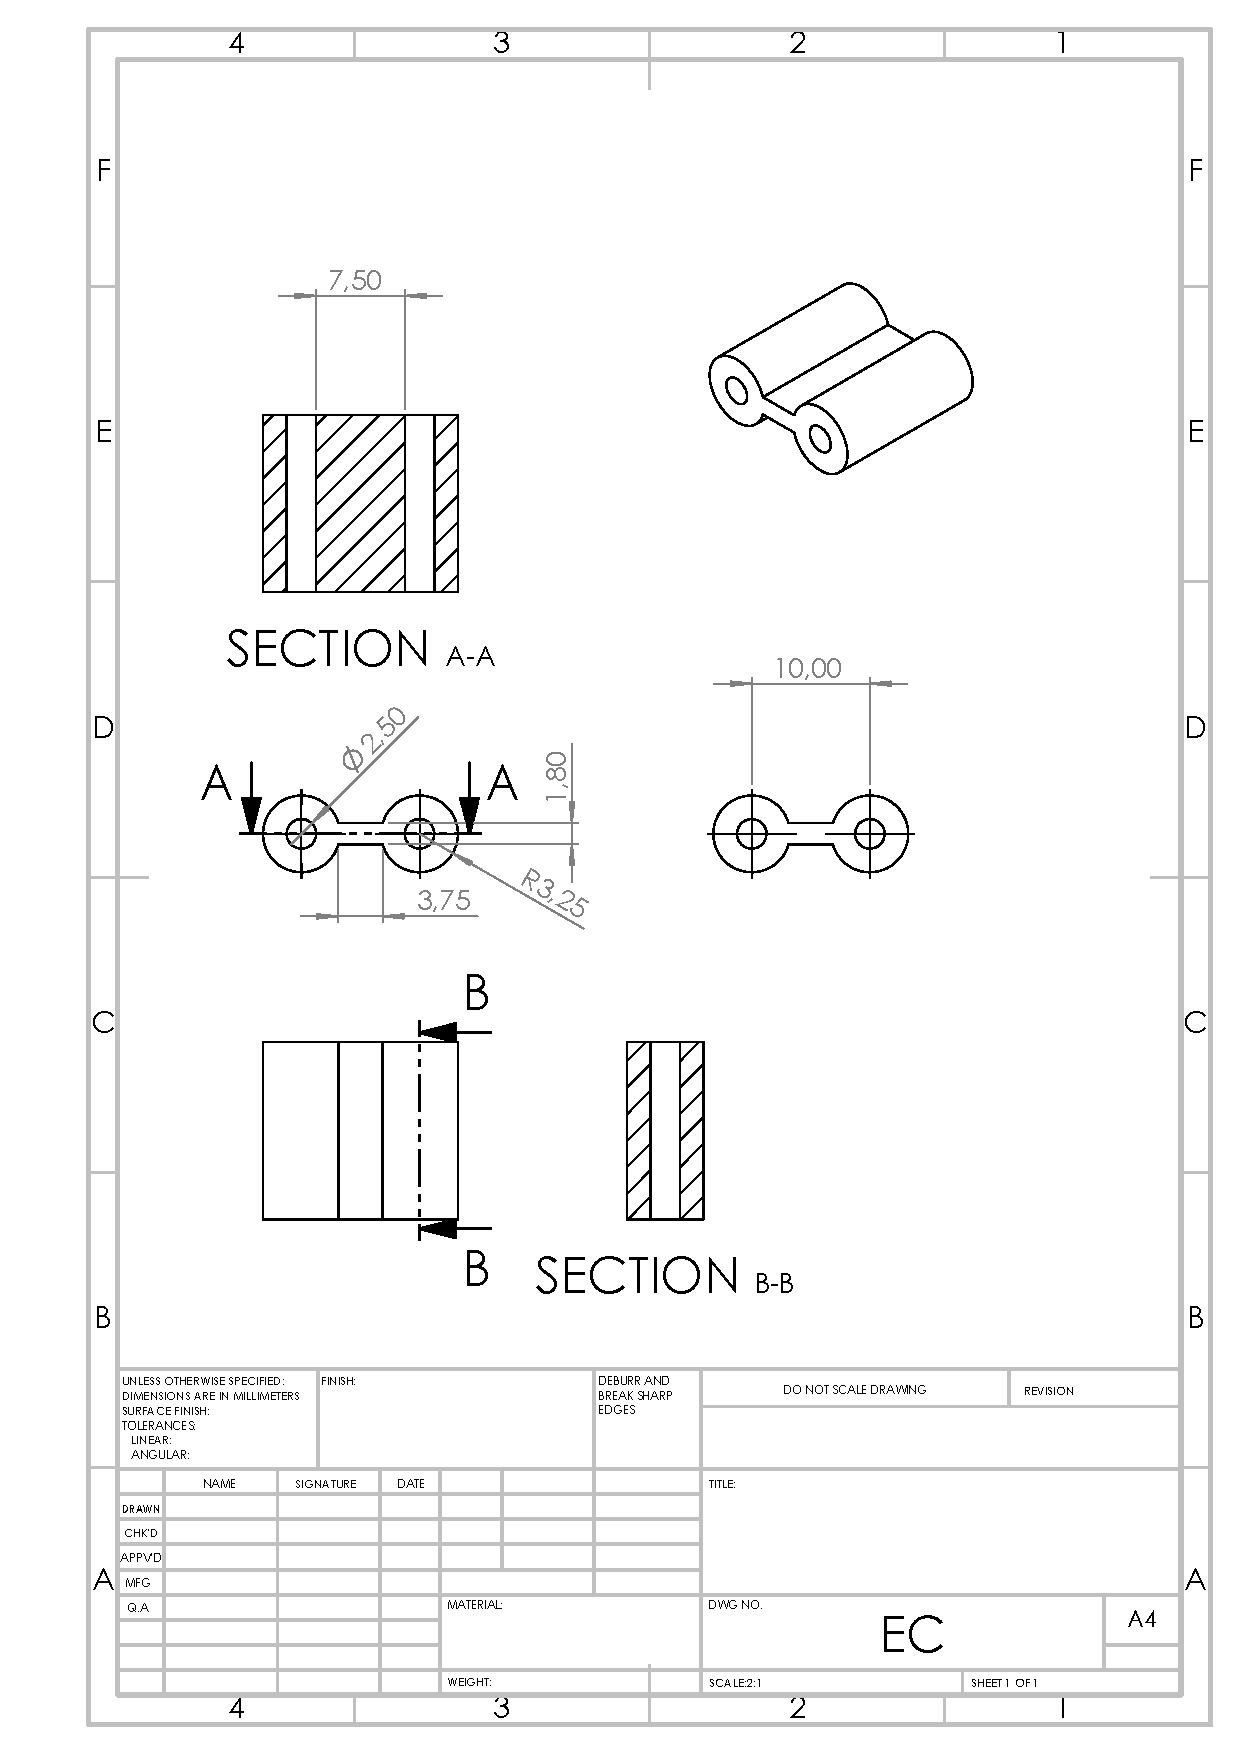
\includegraphics[width=0.62\textwidth]{Embout_EC.pdf}
\schemacap{embout}{Plan de l'embout « EC » (échelle 2:1, cotes en mm) : deux perçages de \qty{2,50}{mm} à \qty{10,00}{mm} d'entraxe, reliés par une fente de \qty{1,80}{mm}.}
\end{figure}

\subsubsection*{Le montage}

Je monte la sonde dans l'ordre qui évite de refaire un travail. On commence par imprimer le tube et l'embout, puis par vérifier qu'une mine glisse dans chaque canal sans forcer : si l'impression a resserré un canal, on le dégage avec le foret. Ensuite on coupe les deux mines à la longueur du tube, soit \qty{66,9}{mm}, plus \qty{15}{mm} côté eau et quelques millimètres côté tête pour le contact, soit environ \qty{87}{mm}, avec la scie fine. On les enfile dans les canaux, de sorte qu'il en dépasse \qty{15}{mm} du côté de la collerette.

On glisse alors l'embout sur les mines, côté tête, pour les maintenir à \qty{10}{mm}. On enroule un fil de cuivre fin, bien serré, autour du haut de chaque mine, avec une goutte de colle conductrice si on en a. Le graphite ne se soude pas : c'est la pression du fil qui fait le contact. Puis on soude chaque fil au câble blindé et on vérifie au multimètre que les deux mines ne se touchent pas.

Enfin on remplit de résine époxy la tête et l'embout, de manière à noyer les fils et les contacts, et on colle les mines dans leurs canaux côté eau pour que l'eau ne remonte pas. On laisse durcir le temps indiqué sur le tube. Seul le graphite doit toucher l'eau.

\begin{attention}
Aucun cuivre ne doit toucher l'eau : il se dissoudrait dans la solution, toxique pour les plantes, et fausserait la mesure. Si un morceau de fil dépasse de la résine, je recommence cette étape.
\end{attention}

% ---------------------------------------------------------------------
\Needspace{8\baselineskip}\subsection{Circuit et mesure}

Cette sous-partie présente d'abord le schéma électrique de la mesure et sa nomenclature. Elle démontre ensuite comment on retrouve la résistance de l'eau à partir de deux lectures, puis décrit le programme de l'Arduino qui fait ces lectures. Elle se termine par l'alternance avec la sonde pH.

\subsubsection*{Le schéma électrique}

Je cherche un montage avec le moins de composants possible. Je relie la broche D5 de l'Arduino à la première mine de la sonde par une résistance de référence $R_1$, et la broche D6 directement à la seconde mine. La broche d'entrée analogique A0 lit la tension au point J, entre $R_1$ et la sonde. Pour inverser le courant, il suffit d'échanger les états de D5 et de D6 : l'une est à \qty{5}{V} pendant que l'autre est à \qty{0}{V}, puis l'inverse.

Je dessine le schéma dans le même style que celui de l'Arduino, en pleine page dans le schéma complet de la tour (page suivante). Je le lis de gauche à droite : l'Arduino (-K2) avec ses broches, puis les composants de la mesure au milieu, puis la sonde de température DS18B20\ix{24} (-B4) à droite. Cette sonde reste sur la broche D2, avec sa résistance de tirage $R_2$ de \qty{4,7}{k\ohm}. Les deux phases du courant sont rappelées sur le schéma. Le courant $I$ représenté est celui de la phase 1.

\schemapaysageC{eagle/schema_complet.pdf}{elcompl}{Schéma électrique complet de la tour (alimentation, commande, capteurs et sonde EC), sur une seule feuille.}

\subsubsection*{La nomenclature}

Chaque repère du schéma renvoie à une ligne du tableau.

\begin{table}[H]
\centering
\small
\begin{tabularx}{\textwidth}{|l|l|l|Y|}
\hline
\textbf{Repère} & \textbf{Désignation} & \textbf{Caractéristiques} & \textbf{Fonction} \\
\hline
-B2 & Sonde de conductivité & Deux mines de graphite 4B & Plonge dans l'eau du bac ; sa résistance $R_w$ dépend de la conductivité. \\
\hline
-B4 & Sonde de température DS18B20\ix{24} & Bus 1-Wire & Donne la température de l'eau pour la compensation. \\
\hline
-K2 & Carte Arduino Uno & Broches D2, D5, D6, A0, \qty{5}{V}, GND & Impose \qty{5}{V} ou \qty{0}{V} sur D5 et D6, lit la tension du point J sur A0 et dialogue avec la sonde de température. \\
\hline
-R1 & Résistance de référence & \qty{340}{\ohm}, 1 \% & Forme avec la sonde un pont diviseur de tension. \\
\hline
-R2 & Résistance de tirage & \qty{4,7}{k\ohm} & Maintient le bus 1-Wire à l'état haut. \\
\hline
-X1 & Bornier du DS18B20\ix{24} & 3 bornes & Raccorde la sonde de température. \\
\hline
\end{tabularx}
\caption{Nomenclature du circuit de mesure de l'EC.}
\end{table}

\subsubsection*{De deux tensions à la résistance de l'eau}

Il me reste à savoir quoi calculer avec les lectures de l'entrée A0. Je mesure la tension au point J dans chacune des deux phases, puis j'en fais le rapport. Je pars de l'hypothèse que chaque broche se comporte comme une source de tension $V$ en série avec une petite résistance : $r_H$ à l'état haut, $r_L$ à l'état bas (en ohms, quelques dizaines d'ohms pour un Arduino).

\naturecalc{théorie (formule démontrée, valeurs de fiches techniques et hypothèses ; rien de mesuré)}
\begin{demonstration}[résistance de l'eau à partir de deux tensions]
\resultat{R_w = R_1 + P\,(x - 1)\quad\text{avec}\quad x = \frac{U_1}{U_2}\ \text{et}\ P = R_1 + r_L}
\textbf{Phase 1 :} D5 à l'état haut, D6 à l'état bas. Le courant traverse, en série, $r_H$, $R_1$, la sonde $R_w$ et $r_L$. Il vaut (en ampères) :
\[
I_1 = \frac{V}{r_H + R_1 + R_w + r_L}
\]
Le point J est situé entre $R_1$ et la sonde. Sa tension $U_1$ (en volts) est la chute de tension dans $R_w$ et $r_L$ :
\begin{align*}
U_1 &= (R_w + r_L)\,I_1\\
U_1 &= V\,\frac{R_w + r_L}{r_H + R_1 + R_w + r_L}
\end{align*}
\textbf{Phase 2 :} D5 à l'état bas, D6 à l'état haut. Le courant traverse $r_H$, la sonde, $R_1$ et $r_L$ : c'est la même somme, donc le même courant, mais en sens inverse :
\[
I_2 = \frac{V}{r_H + R_w + R_1 + r_L} = I_1
\]
Le point J est maintenant situé entre la sonde et $R_1$. Sa tension $U_2$ (en volts) est la chute de tension dans $R_1$ et $r_L$ :
\begin{align*}
U_2 &= (R_1 + r_L)\,I_2\\
U_2 &= V\,\frac{R_1 + r_L}{r_H + R_1 + R_w + r_L}
\end{align*}
Je fais le rapport $x = U_1/U_2$ : $V$, $r_H$ et le dénominateur disparaissent.
\begin{align*}
x &= \frac{U_1}{U_2}\\
x &= \frac{R_w + r_L}{R_1 + r_L}
\end{align*}
J'isole $R_w$ :
\begin{align*}
R_w + r_L &= (R_1 + r_L)\,x\\
R_w &= (R_1 + r_L)\,x - r_L
\end{align*}
Je pose $P = R_1 + r_L$ (en ohms), donc $r_L = P - R_1$ :
\begin{align*}
R_w &= P\,x - (P - R_1)\\
R_w &= R_1 + P\,(x - 1)
\end{align*}
Ce résultat est précieux. Le rapport $x$ ne dépend ni de la tension d'alimentation, ni de la référence du convertisseur, ni de $r_H$. La seule inconnue est $P$, que je mesure à l'étalonnage (partie 7.7). Comme les deux phases font passer le même courant en sens contraire, le courant moyen dans la sonde est nul :
\[
\frac{I_1 + (-I_2)}{2} = 0
\]
ce qui réalise la condition posée à la partie 7.4.
\end{demonstration}

\subsubsection*{Le programme de mesure}

Le Raspberry ne peut pas faire cette mesure lui-même : un aller-retour par le câble USB dure plusieurs millisecondes, alors qu'une phase doit durer environ \qty{130}{\micro s}. Je choisis donc de faire toute la mesure dans l'Arduino, en une seule commande, que j'ajoute au programme \texttt{HydroTour\_Firmata}. Le Raspberry demande la mesure et reçoit en retour les deux sommes $S_1$ et $S_2$. Cette commande a été écrite et installée le 20 novembre 2026 : la partie 9.1 en donne le détail.

L'Arduino répète 64 fois les deux phases. À chaque phase, il attend \qty{20}{\micro s} que la tension se stabilise, puis lit l'entrée A0 et l'ajoute à une somme. Ensuite, il remet les deux broches en entrée pour déconnecter la sonde. Une lecture est un nombre entier de 0 à 1\,023.

L'organigramme suivant résume la commande « mesure EC » dans l'Arduino.

\begin{figure}[H]
\centering
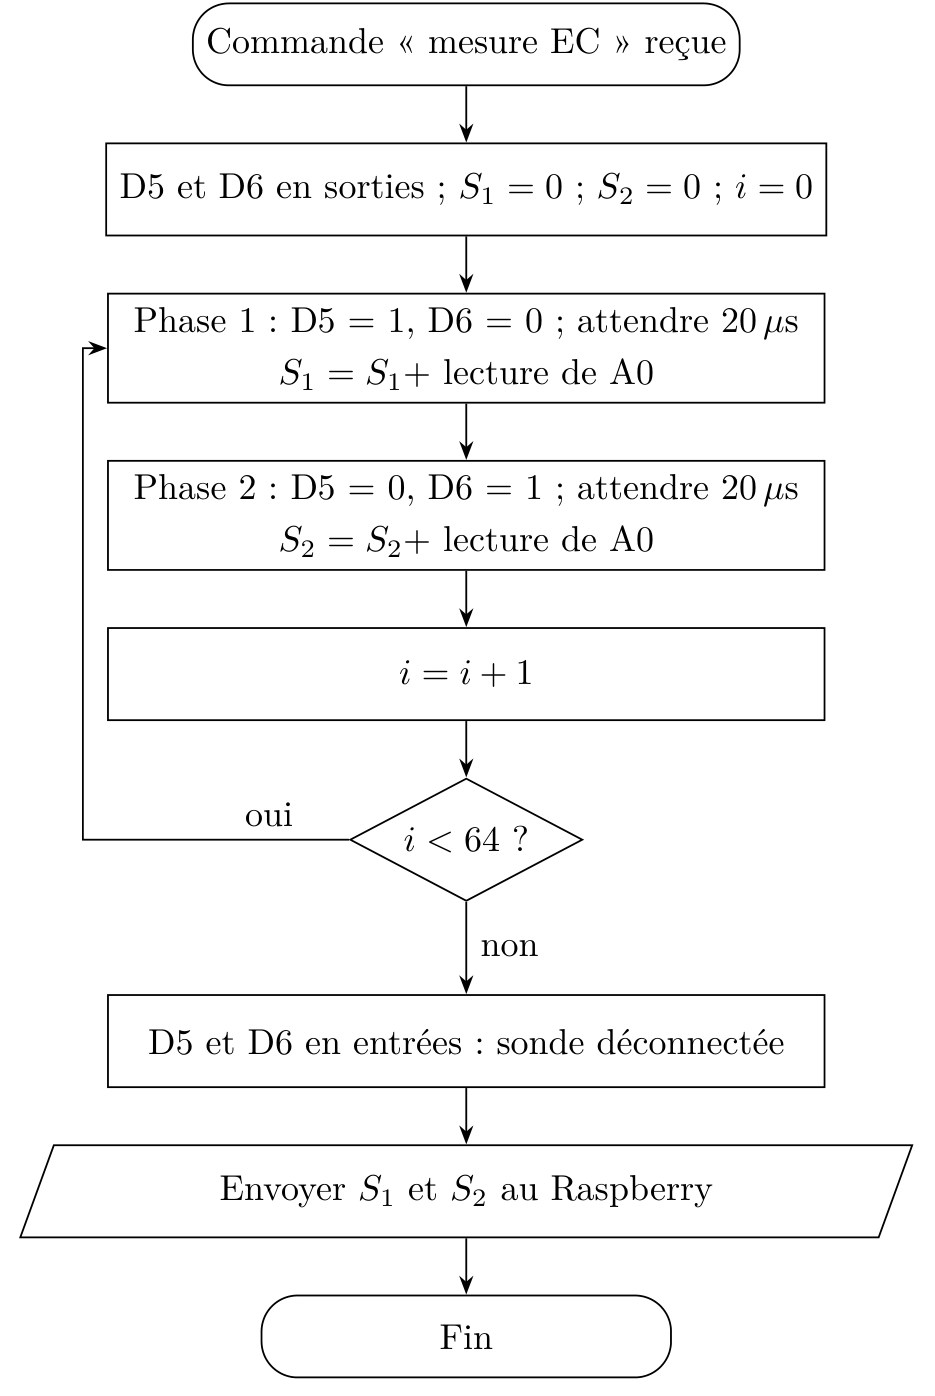
\includegraphics[width=0.5\textwidth]{img/inf/g_orga_ec.png}
\schemacap{orgaec}{Organigramme (ISO 5807) de la commande « mesure EC » dans l'Arduino.}
\end{figure}

\naturecalc{théorie (formule démontrée, valeurs de fiches techniques et hypothèses ; rien de mesuré)}
\begin{demonstration}[durée d'une mesure et taille des sommes]
\resultat{T \approx \qty{17}{ms}\quad\text{et}\quad S_{\max} = 65\,472}
Une phase comprend l'attente de \qty{20}{\micro s} et une lecture analogique, qui dure environ \qty{112}{\micro s} avec le réglage habituel de l'Arduino :
\begin{align*}
t_{\text{phase}} &= \qty{20}{\micro s} + \qty{112}{\micro s}\\
t_{\text{phase}} &= \qty{132}{\micro s} \approx \qty{130}{\micro s}
\end{align*}
Une mesure comprend $64\times 2 = 128$ phases :
\begin{align*}
T &= 128\times\qty{132}{\micro s}\\
T &= \qty{16896}{\micro s}\\
T &\approx \qty{17}{ms}
\end{align*}
Le courant change de sens toutes les \qty{132}{\micro s}, soit une période de \qty{264}{\micro s} (une phase 1 puis une phase 2) et une fréquence de :
\begin{align*}
f &= \frac{1}{\qty{264}{\micro s}}\\
f &\approx \qty{3800}{Hz}
\end{align*}
Chaque somme est au plus égale à 64 lectures de 1\,023 :
\begin{align*}
S_{\max} &= 64\times 1023\\
S_{\max} &= 65\,472
\end{align*}
Cette valeur est inférieure à $65\,535 = 2^{16} - 1$ : un entier de 16 bits suffit pour chaque somme.
\end{demonstration}

Le rapport $x$ se calcule ensuite sur le Raspberry. Les 64 lectures de chaque phase ont la même échelle, donc leur rapport est celui des tensions :
\[
x = \frac{S_1}{S_2} = \frac{U_1}{U_2}
\]

La figure suivante montre l'inversion de la polarité pendant une mesure.

\begin{figure}[H]
\centering
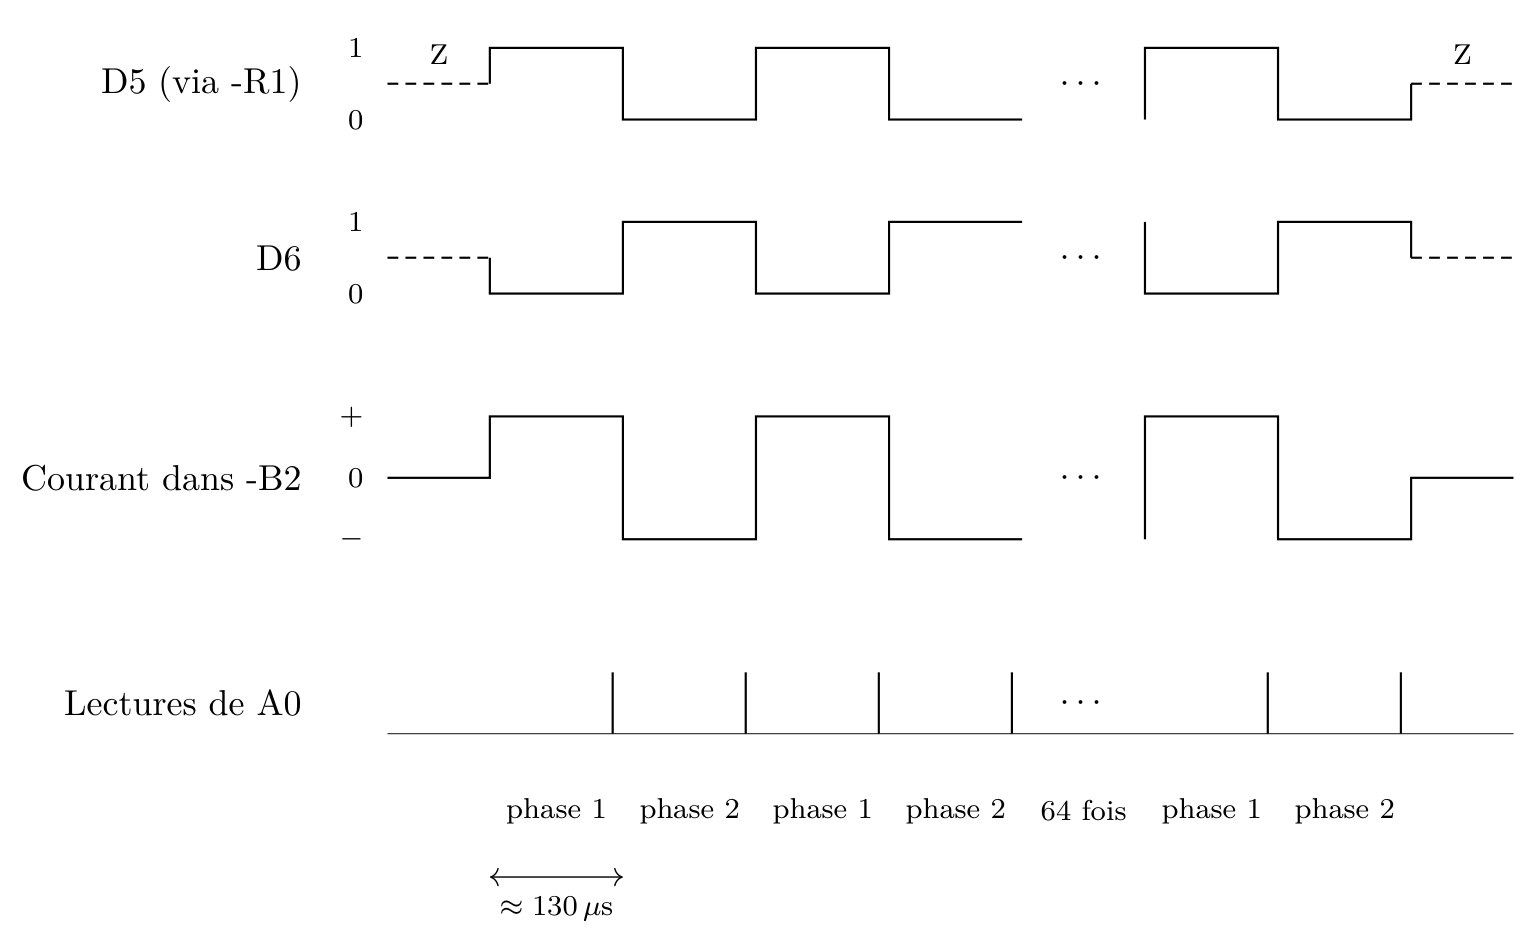
\includegraphics[width=0.92\textwidth]{img/inf/g_inversion.png}
\schemacap{inversion}{Inversion de polarité pendant une mesure. Z : broche en entrée (haute impédance), la sonde n'est reliée à rien.}
\end{figure}

\subsubsection*{L'alternance avec la sonde pH}

Je dois encore m'assurer que la mesure de l'EC ne perturbe pas la sonde pH plongée dans le même bac. Je garde la règle déjà adoptée pour le projet : la carte pH est coupée par la sortie 4 de la carte MOSFET\ix{15} pendant la mesure de l'EC, et le pH n'est pas lu dans les \qty{5}{s} qui suivent. La mesure de l'EC a lieu une fois par minute, alors que le pH est lu toutes les \qty{10}{s} (figure suivante). La lecture du pH prévue à \qty{60}{s} est donc sautée ; la suivante, à \qty{70}{s}, a lieu \qty{9,5}{s} après la mesure.

\begin{figure}[H]
\centering
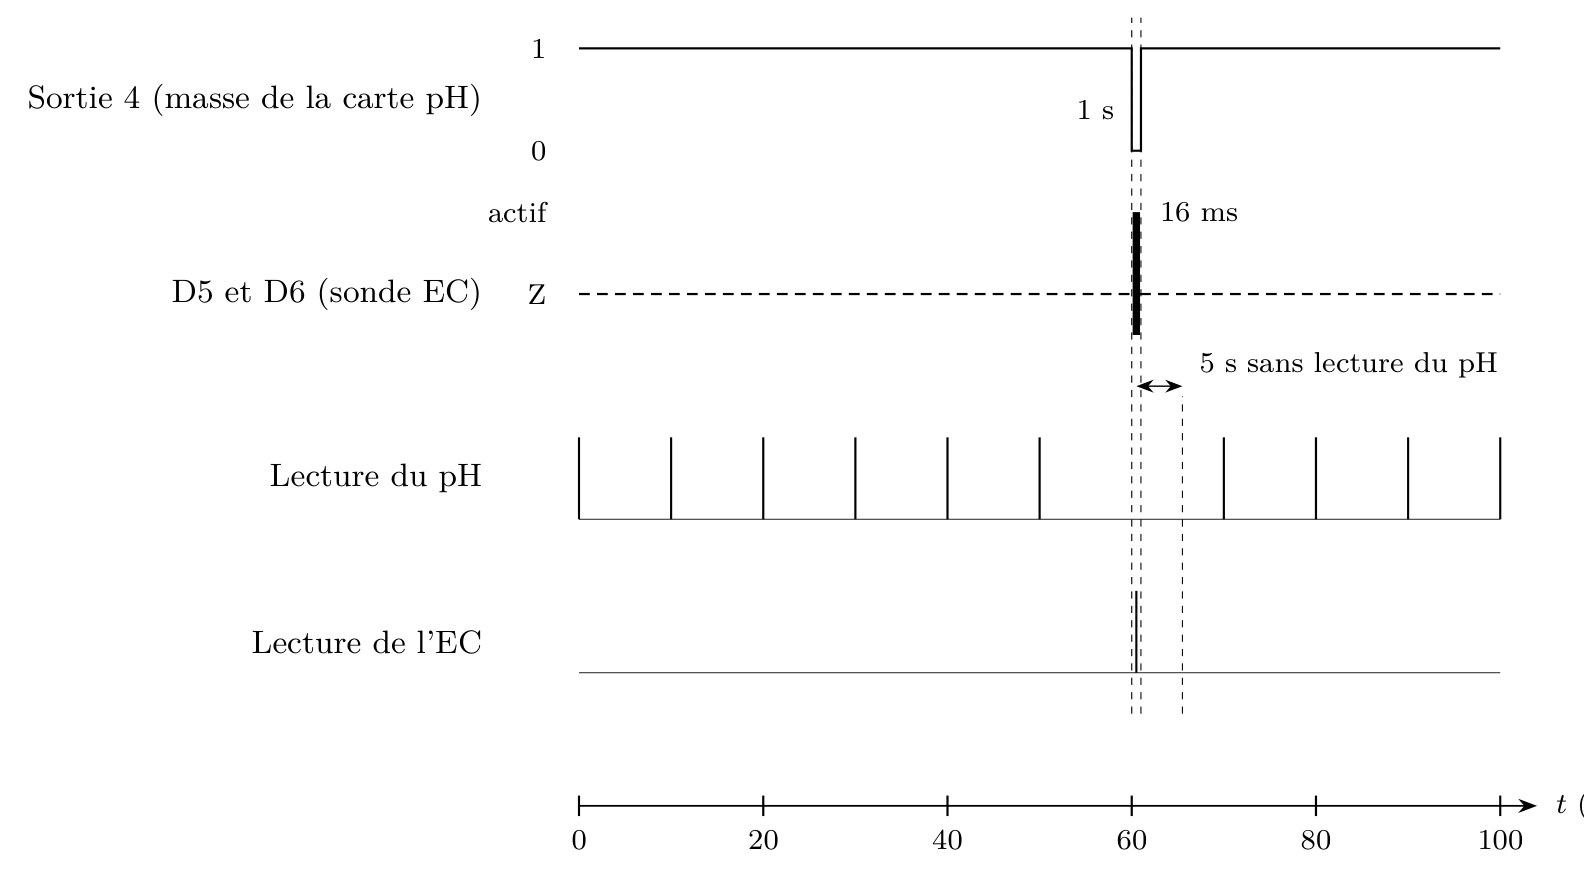
\includegraphics[width=0.92\textwidth]{img/inf/g_deroulement.png}
\schemacap{deroul}{Déroulement sur 100 s : le pH est lu toutes les 10 s, l'EC une fois par minute pendant 16 ms. La sortie 4 coupe la carte pH autour de la mesure.}
\end{figure}

Comme la mesure de l'EC ne dure que \qty{16}{ms} avec un courant moyen nul, ces précautions sont peut-être excessives. Je ne le sais pas : je les garde tant qu'un essai (partie 7.8) ne montre pas qu'on peut les alléger.

\begin{aretenir}
Une mesure de l'EC, c'est 64 allers-retours du courant en environ \qty{17}{ms}, deux sommes $S_1$ et $S_2$ envoyées au Raspberry, et la sonde déconnectée le reste du temps.
\end{aretenir}

% ---------------------------------------------------------------------
\Needspace{8\baselineskip}\subsection{Étalonnage et calcul de l'EC}

Cette sous-partie explique d'abord comment ramener la conductivité à une température de référence. Elle démontre ensuite comment deux solutions étalons donnent la constante de cellule $K$ et la résistance $P$, puis applique le calcul à un exemple chiffré. Elle décrit enfin la procédure d'étalonnage.

\subsubsection*{La température}

La conductivité d'une solution augmente quand elle se réchauffe, car les ions se déplacent plus vite. Le DS18B20\ix{24} donne la température de l'eau ; je ramène chaque mesure à \qty{25}{\celsius}, température de référence des solutions étalons. Pour cela, je suppose que l'augmentation est proportionnelle à l'écart avec \qty{25}{\celsius}, avec un coefficient $\alpha$ d'environ \qty{0,02}{\celsius^{-1}}, soit \qty{2}{\percent} par degré.

\naturecalc{théorie (formule démontrée, valeurs de fiches techniques et hypothèses ; rien de mesuré)}
\begin{demonstration}[conductivité ramenée à \qty{25}{\celsius}]
\resultat{\sigma_{25} = \frac{\sigma_T}{1 + \alpha\,(T - 25)}}
La conductivité $\sigma_T$ mesurée à la température $T$ (en \unit{\celsius}) s'écrit, d'après l'hypothèse, à partir de la conductivité $\sigma_{25}$ à \qty{25}{\celsius} (toutes deux en mS/cm) :
\[
\sigma_T = \sigma_{25} + \alpha\,(T - 25)\,\sigma_{25}
\]
Je mets $\sigma_{25}$ en facteur :
\[
\sigma_T = \sigma_{25}\,\bigl(1 + \alpha\,(T - 25)\bigr)
\]
Je divise par le facteur entre parenthèses :
\[
\sigma_{25} = \frac{\sigma_T}{1 + \alpha\,(T - 25)}
\]
Exemple avec $\sigma_T = \qty{1,20}{mS/cm}$ à $T = \qty{20}{\celsius}$ et $\alpha = \qty{0,02}{\celsius^{-1}}$ :
\begin{align*}
\sigma_{25} &= \frac{\qty{1,20}{mS/cm}}{1 + \qty{0,02}{\celsius^{-1}}\times(\qty{20}{\celsius} - \qty{25}{\celsius})}\\
\sigma_{25} &= \frac{\qty{1,20}{mS/cm}}{1 - 0{,}10}\\
\sigma_{25} &= \frac{\qty{1,20}{mS/cm}}{0{,}90}\\
\sigma_{25} &\approx \qty{1,33}{mS/cm}
\end{align*}
Le dernier signe est $\approx$ car $1{,}20/0{,}90$ ne tombe pas juste : j'arrondis au centième.
\end{demonstration}

\subsubsection*{L'étalonnage avec deux solutions}

Il me reste deux inconnues : la constante de cellule $K$, qui dépend de la forme de la sonde, et la résistance $P = R_1 + r_L$, qui dépend de l'Arduino. Pour les trouver, je plonge la sonde dans deux solutions de conductivité connue : l'une à \qty{1,413}{mS/cm}, proche de la plage de travail, et l'autre à \qty{12,88}{mS/cm}, où la résistance de l'eau est faible et où $r_L$ pèse beaucoup. Chaque solution donne un rapport $x$ et une équation.

\naturecalc{théorie (formule démontrée, valeurs de fiches techniques et hypothèses ; rien de mesuré)}
\begin{demonstration}[constante de cellule $K$ et résistance $P$]
\resultat{P = \frac{R_1\,(\sigma_2 - \sigma_1)}{\sigma_1\,(x_1 - 1) - \sigma_2\,(x_2 - 1)}\quad\text{et}\quad K = \sigma_1\,\bigl(R_1 + P\,(x_1 - 1)\bigr)}
On note $\sigma_1 = \qty{1,413}{mS/cm}$ et $\sigma_2 = \qty{12,88}{mS/cm}$ les conductivités des solutions, et $x_1$ et $x_2$ les rapports $U_1/U_2$ mesurés dedans. D'après la partie 7.6, $R_w = R_1 + P\,(x - 1)$, et d'après la partie 7.5, $R_w = K/\sigma$. Pour chaque solution :
\begin{align*}
\frac{K}{\sigma_1} &= R_1 + P\,(x_1 - 1)\\
\frac{K}{\sigma_2} &= R_1 + P\,(x_2 - 1)
\end{align*}
J'isole $K$ dans la première équation :
\[
K = \sigma_1\,\bigl(R_1 + P\,(x_1 - 1)\bigr)
\]
Je le remplace dans la seconde :
\[
\frac{\sigma_1}{\sigma_2}\,\bigl(R_1 + P\,(x_1 - 1)\bigr) = R_1 + P\,(x_2 - 1)
\]
Je multiplie par $\sigma_2$ :
\[
\sigma_1\,R_1 + \sigma_1\,P\,(x_1 - 1) = \sigma_2\,R_1 + \sigma_2\,P\,(x_2 - 1)
\]
Je regroupe les termes en $P$ d'un côté et les autres de l'autre :
\begin{align*}
\sigma_1\,P\,(x_1 - 1) - \sigma_2\,P\,(x_2 - 1) &= \sigma_2\,R_1 - \sigma_1\,R_1\\
P\,\bigl[\sigma_1\,(x_1 - 1) - \sigma_2\,(x_2 - 1)\bigr] &= R_1\,(\sigma_2 - \sigma_1)\\
P &= \frac{R_1\,(\sigma_2 - \sigma_1)}{\sigma_1\,(x_1 - 1) - \sigma_2\,(x_2 - 1)}
\end{align*}
On en déduit $K$ avec l'expression trouvée plus haut.
\end{demonstration}

Une fois $K$ et $P$ connus, la mesure se fait en trois temps : on calcule $x = S_1/S_2$, puis $R_w = R_1 + P\,(x - 1)$, et enfin $\sigma_T = K/R_w$, que l'on ramène à \qty{25}{\celsius}.

\subsubsection*{Un exemple chiffré}

Pour vérifier que les formules se tiennent, je les applique à des valeurs que je choisis moi-même. Ce ne sont pas des mesures : elles servent seulement à contrôler le calcul. Je suppose $K = \qty{1,200}{cm^{-1}}$, $r_L = \qty{25}{\ohm}$ et $R_1 = \qty{330}{\ohm}$, donc $P = \qty{355}{\ohm}$. Ces trois valeurs sont choisies pour l'exemple et ne sont pas celles du montage : la résistance réellement montée vaut \qty{340}{\ohm}. Seul le déroulement du calcul compte ici.

\begin{exemple}[retrouver $K$ et $P$ à partir de $x_1$ et $x_2$]
Dans la solution à \qty{1,413}{mS/cm}, la résistance de l'eau serait :
\begin{align*}
R_{w1} &= \frac{K}{\sigma_1} = \frac{\qty{1,200}{cm^{-1}}}{\qty{1,413e-3}{S/cm}}\\
R_{w1} &\approx \qty{849,3}{\ohm}
\end{align*}
Le rapport correspondant, d'après $x = (R_w + r_L)/(R_1 + r_L)$, vaut :
\begin{align*}
x_1 &= \frac{\qty{849,3}{\ohm} + \qty{25}{\ohm}}{\qty{355}{\ohm}}\\
x_1 &\approx 2{,}463
\end{align*}
Dans la solution à \qty{12,88}{mS/cm} :
\begin{align*}
R_{w2} &= \frac{\qty{1,200}{cm^{-1}}}{\qty{12,88e-3}{S/cm}} \approx \qty{93,2}{\ohm}\\
x_2 &= \frac{\qty{93,2}{\ohm} + \qty{25}{\ohm}}{\qty{355}{\ohm}} \approx 0{,}333
\end{align*}
Je retrouve $P$ avec la formule démontrée :
\begin{align*}
P &= \frac{\qty{330}{\ohm}\times(\qty{12,88}{mS/cm} - \qty{1,413}{mS/cm})}{\qty{1,413}{mS/cm}\times(2{,}463 - 1) - \qty{12,88}{mS/cm}\times(0{,}333 - 1)}\\
P &= \frac{\qty{330}{\ohm}\times\qty{11,467}{mS/cm}}{\qty{2,067}{mS/cm} + \qty{8,591}{mS/cm}}\\
P &= \frac{\qty{3784}{\ohm.mS/cm}}{\qty{10,658}{mS/cm}}\\
P &\approx \qty{355}{\ohm}
\end{align*}
Puis $K$ :
\begin{align*}
K &= \qty{1,413}{mS/cm}\times\bigl(\qty{330}{\ohm} + \qty{355}{\ohm}\times(2{,}463 - 1)\bigr)\\
K &= \qty{1,413}{mS/cm}\times\qty{849,4}{\ohm}\\
K &\approx \qty{1200}{\ohm.mS/cm}
\end{align*}
Comme $\qty{1}{mS}\times\qty{1}{\ohm} = \num{e-3}$ (en siemens fois ohm, sans unité), on obtient $K \approx \qty{1,200}{cm^{-1}}$, la valeur de départ.

Si la sonde donne ensuite $x = 1{,}50$ dans la solution du bac :
\begin{align*}
R_w &= \qty{330}{\ohm} + \qty{355}{\ohm}\times(1{,}50 - 1)\\
R_w &= \qty{330}{\ohm} + \qty{177,5}{\ohm}\\
R_w &= \qty{507,5}{\ohm}\\
\sigma &= \frac{K}{R_w} = \frac{\qty{1,200}{cm^{-1}}}{\qty{507,5}{\ohm}}\\
\sigma &\approx \qty{2,36e-3}{S/cm} = \qty{2,36}{mS/cm}
\end{align*}
\end{exemple}

\subsubsection*{La procédure d'étalonnage}

Je prévois d'étalonner dans cet ordre, pour ne pas contaminer une solution avec l'autre. On rince d'abord la sonde à l'eau déminéralisée et on l'essuie sans frotter, puis on la plonge dans la solution à \qty{1,413}{mS/cm} en attendant que la température se stabilise. Ensuite on laisse le Raspberry enregistrer plusieurs mesures de suite et on en garde la moyenne, qui donne $x_1$. On rince de nouveau la sonde, on recommence avec la solution à \qty{12,88}{mS/cm}, ce qui donne $x_2$. Le Raspberry calcule alors $K$ et $P$ avec la formule de la partie 7.7 et les enregistre, comme il le fait déjà pour le pH.

Pour contrôler le résultat, on replonge la sonde dans la solution à \qty{1,413}{mS/cm} : la valeur affichée doit s'en approcher à quelques pour cent près. Les boutons d'étalonnage de l'EC ne sont pas encore dans le dashboard.

\begin{attention}
Les solutions étalons sont données pour \qty{25}{\celsius}. Si elles sont à une autre température, j'applique la même compensation qu'à la partie 7.7 avant de calculer $K$ et $P$.
\end{attention}

% ---------------------------------------------------------------------
\Needspace{8\baselineskip}\subsection{Essais et limites de la sonde EC}

Cette sous-partie dit d'abord ce qui est vérifié aujourd'hui, puis les essais que je prévois sur la vraie sonde. Elle se termine par un tableau de synthèse de l'état d'avancement.

\subsubsection*{Ce qui est vérifié}

Je préfère être clair : à ce jour, aucune mesure n'a été faite avec cette sonde. L'étude de conception est terminée : la géométrie, le circuit, les calculs et le déroulement de la mesure sont posés et démontrés. La sonde n'est pas construite, la commande n'est pas écrite dans l'Arduino et aucun étalonnage n'a été fait. Les exemples chiffrés de la partie 7.7 sont des valeurs que j'ai choisies, pas des mesures.

\subsubsection*{Les essais prévus}

Je prévois de tester la sonde étape par étape, dans l'ordre où les erreurs coûtent le moins cher. On commence par vérifier au multimètre, avant de verser la résine, que les deux mines ne se touchent pas. Une fois la sonde terminée, on la plonge dans la solution à \qty{1,413}{mS/cm} et on compare la résistance de l'eau calculée à la plage attendue de la partie 7.5. Ensuite on étalonne avec les deux solutions, puis on vérifie la répétabilité : dix mesures de suite dans la même solution doivent donner presque la même valeur.

Il faut ensuite mesurer l'effet sur le pH : on lit le pH dans une solution tampon avec, puis sans mesure de l'EC dans le même bac. Si l'écart est négligeable, on peut alléger la coupure de la carte pH de la partie 7.6. Enfin, on refait l'étalonnage après une semaine dans la solution nutritive, pour savoir si la sonde en graphite dérive ou s'encrasse, et à quelle fréquence il faut la nettoyer.

\begin{attention}
Un ohmmètre de multimètre travaille en courant continu : dans l'eau, il affiche une valeur qui dérive (partie 7.4). Il ne sert qu'à détecter un court-circuit, jamais à mesurer la résistance de l'eau.
\end{attention}

\subsubsection*{Synthèse}

Ce tableau reprend chaque fonction de la sonde avec la solution retenue et son état.

\begin{table}[H]
\centering
\small
\begin{tabularx}{\textwidth}{|l|Y|l|}
\hline
\textbf{Fonction} & \textbf{Solution retenue} & \textbf{État} \\
\hline
Électrodes & deux mines de graphite 4B de \qty{1,8}{mm}, entraxe \qty{10}{mm}, tube et embout imprimés en 3D & plans dessinés \\
\hline
Courant alternatif & inversion de polarité à environ \qty{3800}{Hz} & programmé \\
\hline
Circuit & $R_1 = \qty{340}{\ohm}$, broches D5 et D6, lecture sur A0 & monté \\
\hline
Conversion en $R_w$ & rapport $x = S_1/S_2$ puis $R_w = R_1 + P\,(x-1)$ & démontré \\
\hline
Commande de mesure & 64 allers-retours, sommes $S_1$ et $S_2$ & écrite et installée (partie 9.1) \\
\hline
Température & compensation à \qty{25}{\celsius}, $\alpha = \qty{0,02}{\celsius^{-1}}$ & démontré \\
\hline
Étalonnage & deux solutions, conductivités au choix & écrit, essai à faire \\
\hline
Sonde pH & carte coupée pendant la mesure, pas de lecture dans les \qty{5}{s} & à essayer \\
\hline
\end{tabularx}
\caption{Synthèse de la sonde EC fabriquée.}
\end{table}

\begin{aretenir}
La conception est complète. La commande de mesure est écrite et donne sa première valeur dans l'eau depuis le 20 novembre 2026 (partie 9.4), mais la sonde n'est pas encore étalonnée : il reste à faire l'étalonnage à deux solutions avant de pouvoir parler de précision.
\end{aretenir}

